\section{Introduction}\label{sec:intro}
\sectionstate{partial}{v2 2026-11-10: results paragraph and the two-tracks paragraph are new, the rest is the paper1 text; drafted 2026-11-06 from Dylan's note, revised the same day from his comments; kinematics from $Q=20.58$\,MeV and $m_X=16.8$\,MeV; air scattering: Highland formula, 204\,mm of air; stack distances from the surveyed Geant4 geometry (\texttt{MX17\_Full\_Geant/include/SimConfig.hh})}

In 2016 the ATOMKI group reported an excess of $e^+e^-$ pairs at large opening angles in the decay of an excited
state of $^8$Be~\cite{Krasznahorkay2016}, and later in $^4$He~\cite{Krasznahorkay2021} and
$^{12}$C~\cite{Krasznahorkay2022}. All three are consistent with the emission of a light neutral boson of mass
${\approx}17$\,MeV that decays to $e^+e^-$, now called X17~\cite{Feng2016}. Independent tests have not settled the question:
a two-arm spectrometer in Hanoi reports the $^8$Be anomaly~\cite{Anh2024}; NA64 excludes part of the couplings
favoured by it~\cite{NA64_2018,NA64_2020}; MEG~II, repeating the $^8$Be measurement, sees no significant signal yet
remains compatible with ATOMKI at the 1.5$\sigma$ level~\cite{MEGII2024}; and PADME, searching for X17 produced
resonantly in $e^+e^-$ annihilation, sees an excess of about 2$\sigma$ at $\sqrt{s}\approx16.9$\,MeV~\cite{PADME2025}.
An experiment proposed at the CERN n\_TOF facility~\cite{nTOFX17proposal,Gustavino2025} reaches the $^4$He case with
neutrons instead of protons: capture on $^3$He forms $^4$He 20.58\,MeV above its ground state, which decays by
$\gamma$ emission, by internal pair creation (IPC) or, possibly, by emitting an X17~\cite{Viviani2022}. This paper
describes the compact resistive Micromegas TPCs built to track the leptons from that reaction.

\paragraph{What the measurement needs.}
The experiment must detect the $e^+e^-$ pairs from the hypothetical rare decay of the X17 and reconstruct each
lepton's trajectory from the target. From the kinematics, each lepton carries between about 3 and 16\,MeV. The
opening angle of the pair is related to its invariant mass, which provides the separating power against the smooth
IPC background. The figure of merit of the tracking is therefore the accuracy of each reconstructed track angle.
At these distances a position resolution of the order of a millimetre is enough (\cref{sec:requirement}), and the time
resolution serves only to reject combinatorial background. Tracking is the
first layer of the experiment. Behind it, scintillators trigger and measure the energy, which adds the energy split
of the pair to the mass and rejects events whose total energy is not that of the capture. The tracker must therefore
put as little material as possible in front of its own measurement, and then measure the track well.

\paragraph{Why a compact TPC.}
A Micromegas~\cite{Giomataris1996} time projection chamber was chosen to fill the role of a low-material-budget
tracker. Leptons cross a thin window into a gas volume, and the drift times of the ionisation along each track give
a three-dimensional segment, hence a direction, from a single chamber (\crefp{fig:layout}{b}). The trackers must sit
close to the target, since the air in between scatters the leptons: over 20\,cm an 8\,MeV electron is deflected by
1.7\textdegree{} rms in each projection (3.2\textdegree{} at 4\,MeV), already comparable to the chamber's own angular
resolution. Four chambers therefore form a box around the target, with their entrance windows 20\,cm from it
(\crefp{fig:layout}{a}), each with an active area of about $40\times36$\,cm$^2$, for a large acceptance to the
back-to-back pairs. The trigger and calorimetry scintillators must fit close behind each chamber, the first layer
11\,cm behind the window and the whole stack within about 50\,cm of the target, and this is what makes the chambers
compact, with a 30\,mm drift gap.

\paragraph{Why resistive strips.}
n\_TOF operates in pulsed mode and the instantaneous intensity was expected to be high, so the chambers were built as
resistive Micromegas~\cite{Alexopoulos2011} for survivability and stability. This appears to have worked
(\cref{sec:efficiency}). The resistive strips, however, spread the charge of each avalanche over neighbouring strips
with delay, which poses novel problems for the TPC reconstruction. Reconstruction algorithms for resistive
Micromegas TPCs are discussed here where they affect the performance (\cref{sec:reco}), and in a companion paper
devoted to them~\cite{paperII}.

\paragraph{Two tracks in one chamber.}
\askDylan{New (2026-11-10). \Cref{fig:layout} draws the pair in two chambers, so without this sentence a reader does not
know why \cref{sec:twoparticle} matters. Check the framing: is ``pairs of small opening angle cross one chamber'' the
case you want to make (IPC normalisation, conversions), or something else?}
A pair with a large opening angle, as expected from an X17, crosses two chambers (\crefp{fig:layout}{a}). The far more
numerous pairs of small opening angle from the IPC continuum often cross a single chamber together. A chamber must
therefore also separate two tracks and assign the two segments it sees in each readout view to the right particle.

\paragraph{This paper.}
It covers the chambers themselves, characterised on the Saclay cosmic bench and in the CERN SPS H4 beam; the n\_TOF
campaign and its physics are reported separately. The main results are these. On cosmic muons a single chamber
measures the angle of a track to 1.0\textdegree{} in one view and 0.9\textdegree{} in the other, with no dependence on
the angle within the $\pm20$\textdegree{} the bench provides, on the gain over an order of magnitude or on the drift
field (\cref{sec:tracking}). The chamber calibrates its own drift velocity and drift gap from the data, in two
independent ways that agree to 2\,\%, and so monitors the water and oxygen in its gas (\cref{sec:gas}). The best
chamber detects 94.8\,\% of single tracks over its full active area, and all but 0.6 percentage points of the loss is
real ionisation that a straight-track reconstruction does not describe (\cref{sec:efficiency,sec:straight}). The two
readout views carry equal charge, which pairs the segments of two particles correctly in 97.7\,\% of events, and two
tracks more than 18\,mm apart are both reconstructed in 95\,\% of cases (\cref{sec:twoparticle}). Of five chambers built, two reach this performance and three show production defects
(\cref{sec:conclusions}).

\Cref{sec:requirement} shows why the angle is the quantity to measure. \Cref{sec:design} describes the design and
construction of the chambers, and \cref{sec:setups} the two test setups, the data sets and the reconstruction. The
results follow the measurement: the drift velocity and the gas (\cref{sec:gas}), the angle, position and time
resolution (\cref{sec:tracking}), the operating point and the efficiency (\cref{sec:efficiency}), two particles in one
chamber (\cref{sec:twoparticle}), what a straight-track reconstruction misses (\cref{sec:straight}), and the chamber
as built: a bow of the readout boards and the field fringe at the chamber sides (\cref{sec:asbuilt}).

\begin{figure}[tbp]
  \centering
  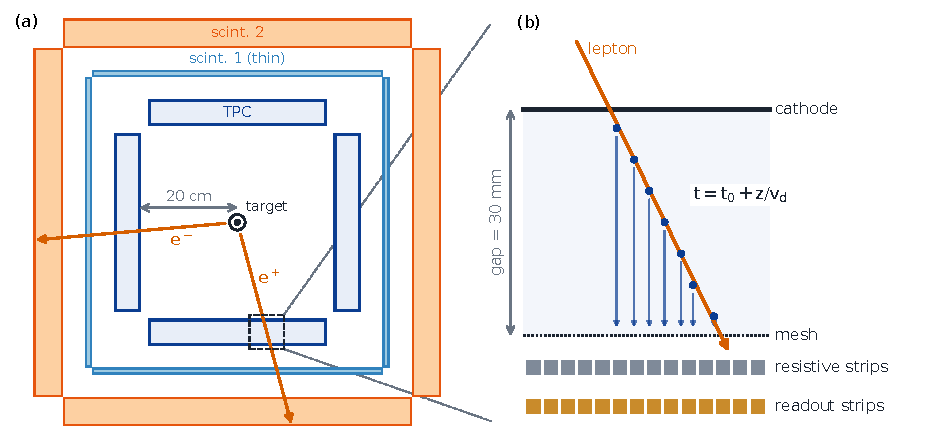
\includegraphics[width=\linewidth]{experiment_layout}
  \caption{The measurement the chambers were built for, schematic. (a) Top-down view, the beam into the page: four
  TPCs form a box around the target, their entrance windows 20\,cm from it, each followed by a thin scintillator
  layer and a thicker one covering the full acceptance (an idealised design); one $e^+e^-$ pair is drawn. (b) The boxed region in section, enlarged (target at the top, gap drawn
  at its nominal 30\,mm; the stage below the mesh enlarged further): the ionisation left along the track drifts
  straight down to the mesh and arrives later the higher it started, $t=t_0+z/\vd$, with $\vd$ the drift velocity; the avalanche lands on the
  resistive strips, which couple it to the readout strips below.}
  \label{fig:layout}
\end{figure}
